\label{chapter: introduction}

% Handwritten page I 


\subsection{What is active matter?}

\todo[inline]{Re-draw figures}

A general definition of active matter is that it is made of elementary units that locally dissipate energy in a continuous and sustained manner. Hence, the dynamics of active particles break time-reversal symmetry, \textit{it is inherently far from thermodynamic equilibrium}. In many cases, activity manifests as persistent motion, but can also take the form of local production of forces, sustaining of chemical reactions, growth (reproduction), or several of them at the same time. This definition is very broad and encompasses a multitude of biological examples spanning many scales:

\begin{figure}[!htb]
    \centering
    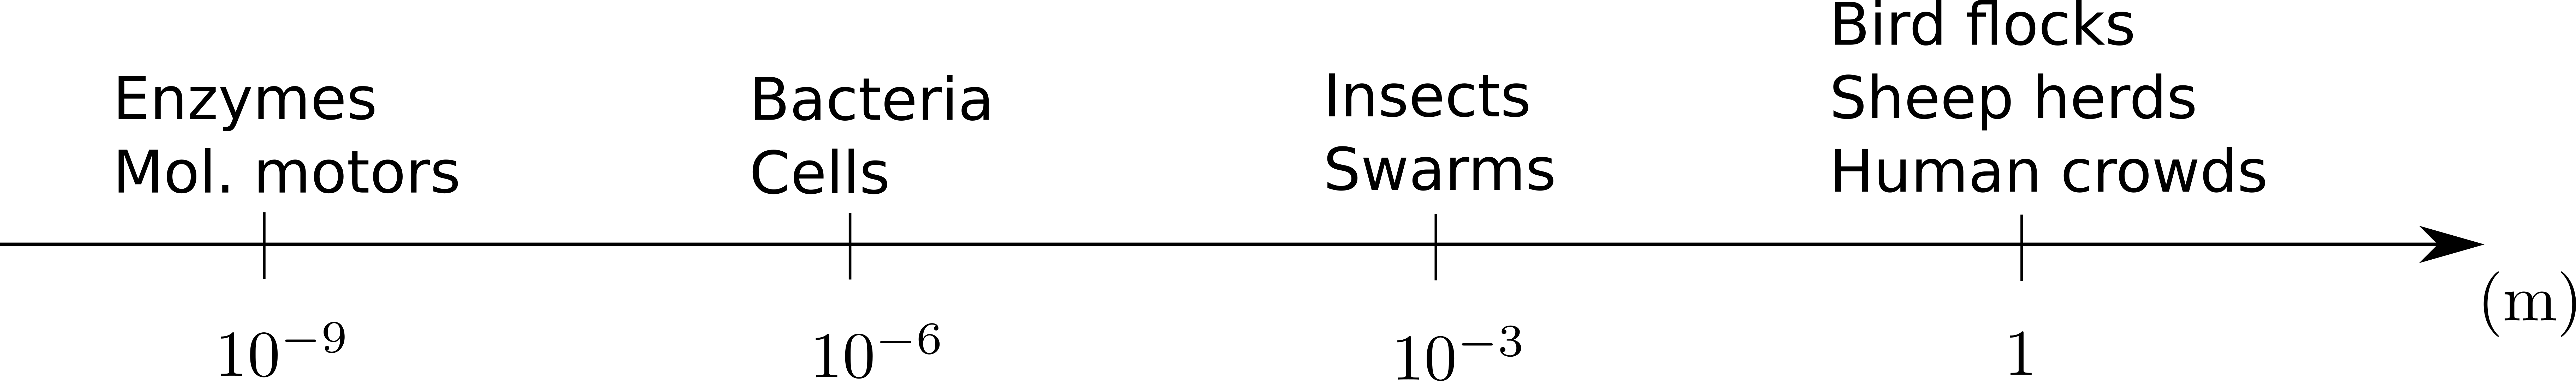
\includegraphics[width=.8\textwidth]{Figures/introduction/scales.png}
    \caption{The range of scales of active particles.}
    \label{fig: scales active particles}
\end{figure}


% Handwritten page II
Some examples of active systems are:

\begin{itemize}
    \item Enzymes and molecular motors, that evolve over the nanometer scale. Enzymes (E) catalyze chemical reactions of their substrate (S) into some product(s) (P),
    %
    \begin{align}
        E + S \longrightarrow  \underbrace{SE}_{\mathrm{binding}} \longrightarrow  E + P,
    \end{align}
    %
     and thus locally sustains chemical gradients $\bm \nabla S$ and $\bm \nabla P$. 
     \begin{figure}[H]
        \centering
        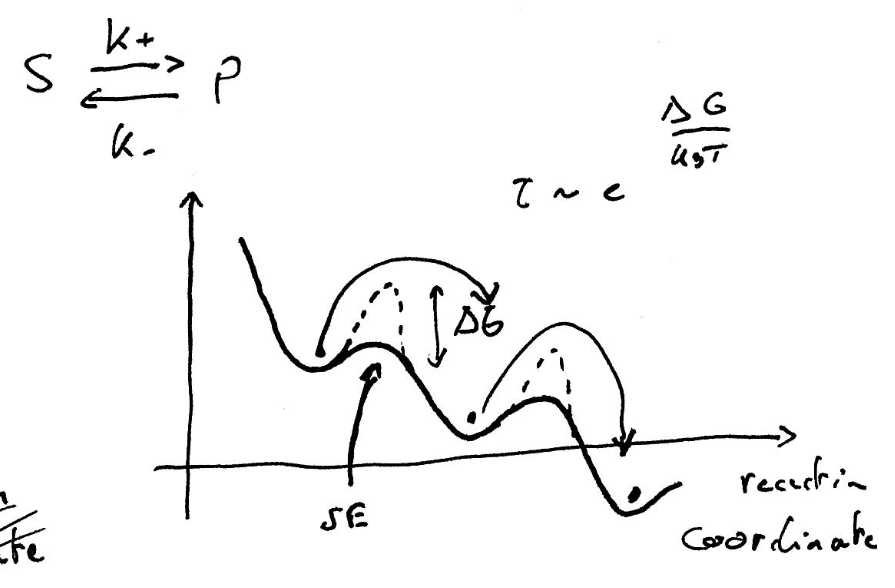
\includegraphics[width=.3\textwidth]{Figures/introduction/enzymes.png}
        \caption{A sketch of how an enzyme works. By various means, the enzyme lowers the effective free energy barrier associated with the $S \to P$ reaction. In the case where a constant supply of substrate is provided, the effect of the enzyme will therefore materialize in the production of chemical currents in some reaction coordinate space.}
        \label{fig: enzymes}
    \end{figure}
    
     Molecular motors are a particular kind of enzyme for which chemical cycles are coupled to displacements or rotations, so that these molecular machines can perform work and, e.g., self-propel.
     \begin{figure}[!htb]
        \centering
        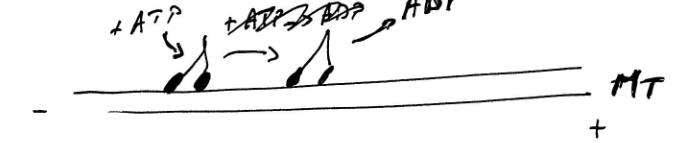
\includegraphics[width=.4\textwidth]{Figures/introduction/motors.png}
        \caption{Molecular motors consume ATP to travel along microtubules.}
        \label{fig: motors}
     \end{figure}
    \item Microorganisms and cells. Bacteria and algae usually move thanks to filamentous appendices called flagella or cilia, which are powered by molecular motors.
    Thanks to their internal machinery, these organisms are therefore able to displace the fluid around them, resulting in a self-propelled motion.
    Another example of self-propulsion at the micrometer scale can be found in some types of cells that are able to glide on substrates by performing cycles of polymerization and depolymerization of actin filaments.
    \\
    \begin{figure}[!htb]
        \centering
        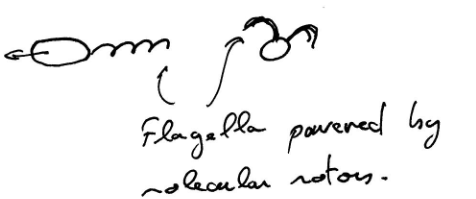
\includegraphics[width=.3\textwidth]{Figures/introduction/bacteria.png} 
        \hspace{2cm}
        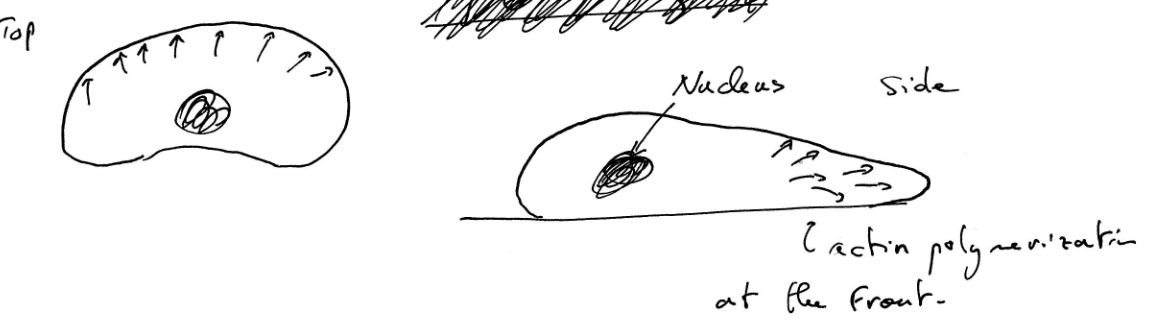
\includegraphics[width=.22\textwidth]{Figures/introduction/actin.png}
        \caption{Motion at a microscopic level: to the left, microswimmers move using flagella. These configurations are called pullers and pushers. To the right, a cell moves by polymerizing acting.}
        \label{fig: label}
    \end{figure}
     
    \item Many familiar examples of active entities are found at larger scales, this incluces e.g. insect swarms at the millimeter scale, and animal herds or human crowds at (roughly) the meter scale.
\end{itemize}


% Handwritten page III

\subsection{What makes active matter special?}

Active systems, because they constantly dissipate energy at the level of their elementary constituents, 
%and in contrast to passive systems globally driven (for example turbulent flows, shaken granulars, \ldots), 
are able to spontaneously self-assemble into complex and dynamic structures. 
Again, these ideas are relevant to many examples in the living world including the architecture of the cytoskeleton, the morphogenesis of multicellular organisms, or the collective motion arising from social interactions in groups of several hundred or thousands of individuals. 

Active matter is also not restricted to the study of biological systems, as the design and study of synthetic active particles now represent a large part of the field. Those allow for better controlled experiments and often exhibit similar phenomenology as their biological counterpart, thus opening the way to biomimetic materials engineering. 
Famous examples of artificial active matter include assemblies of self-propelled colloids (Phoretic Janus particles, so-called Quincke rollers), artificial microswimmers (self-propelled drops, magnetic swimmers), and robots~\cite{BechingerRMP2016}.

\begin{figure}[!htb]
    \centering
    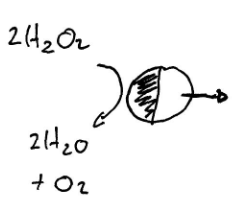
\includegraphics[width=.2\textwidth]{Figures/introduction/janus.png}
    \caption{A self-propelled Janus particle, to be discussed in Chapter~\ref{chap_phoretic}.}
    \label{fig: janus}
\end{figure}



\subsection{On the nonequilibriumness of active assemblies}

As written above, active matter is inherently `far' from equilibrium, since it is assembled from particles whose dynamics constantly break time-reversal symmetry. This means that active systems lack most of the properties on which our intuition of systems at thermodynamic equilibrium is based. These include:
%
\begin{enumerate}
    \item \textit{Absence of minimization principle:} active dynamics are not constrained by the second law of thermodynamics, so that they do not converge over long times to a state of maximal entropy (or minimum free energy). In fact, there is no general argument telling us whether the dynamics of a many-body active system converges to a steady state or not.
    \item \textit{No time-reversal symmetry (TRS):} as a consequence of the previous point, active systems can (and do) generally produce macroscopic currents, leading to phases where TRS is collectively broken.
    \item \textit{Lack of a thermodynamic framework:} Basic equilibrium concepts such as temperature or thermodynamic pressure are usually not defined for active systems. Additionally, active systems generally do not exhibit an equation of state, meaning that their bulk behavior is not only determined by their material properties, but can also be substantially affected by the nature and shape of the container they live in.
    \item \textit{The presence of memory:} again due to 1, and contrary to systems at equilibrium, the state of an active system may be dependent of its past history.
    \item \textit{Emergence of nonreciprocal couplings:} In active matter, momentum is not conserved so forces do not necessarily need to satisfy the action-reaction principle. Familiar examples of such `nonreciprocity' are encountered in predator-prey dynamics, while it also generally arises when particles interact via self-generated fields such as bacteria or phoretic colloids.
    The consequences of the presence of such couplings will be explored in chapter~\ref{chap_nrch}.
\end{enumerate}
%
In summary, the collective behaviors found in active systems generally break our intuition built on equilibrium physics, and their theoretical understanding requires to use and develop tools and concepts specifically tailored to address nonequilibrium dynamics.
In chapter~\ref{chap_thermo}, we will see how field theory descriptions of active systems can be obtained phenomenologically from the framework of irreversible thermodynamics, while coarse-graining techniques will be discussed in chapter~\ref{chap_scalar}.


% Handwritten Page IV

\subsection{The idea of this course}

Active matter is very large and quickly developing field, borrowing tools and concepts from various other areas of physics including soft matter, biological physics, hydrodynamics, and statistical physics. Hence, this course is only meant as an introduction to the basics of the very diverse of active systems, and how it is usually apprehended. In particular, our journey will be driven by two general questions which are still the topic of ongoing research:
\begin{itemize}
    \item How is active motion generated at the micro scale, and what are its consequences on the dynamics of active particles?
    \item How do active systems convert energy dissipated at the molecular scale into the formation of structure and order macroscopic scales?
\end{itemize}
This first chapter is meant to give an overview of the topics that will be addressed in the following lectures, while we will also introduce physics concepts and mathematical tools that will be useful throughout these notes.

% Handwritten page V

\section{Hydrodynamics of microswimmers}

Many (if not most) active particles evolve in a fluid, which they need to displace in order to move. Understanding the locomotion of such swimmers thus requires to study the dynamics of the flow around them. The fluid surrounding the particles is generally incompressible, so that it is defined by its local velocity $\bm v$ which obeys the Navier-Stokes (NS) equations:
%
\begin{subequations}
\label{eq_NS}
\begin{align}
    \label{eq_NS_v}
    \rho \left[ \partial_t \bm v + (\bm v \cdot \nabla)\bm v \right] & = \eta \nabla^2\bm v - \nabla P + \bm f, \\
    \label{eq_NS_inc}
    \nabla \cdot \bm v & = 0.
\end{align}
\end{subequations}
%
The terms on the left-hand side of~\eqref{eq_NS_v} correspond to the material derivative and simply model the effect of inertia, while on the right-hand side the first term originates from viscous dissipation, the second is the pressure which ensures incompressibility as required by~\eqref{eq_NS_inc}, while the active force $\bm f$ arises as a source term.
In cases dominated by inertia or dissipation, the NS Eq.~\eqref{eq_NS} simplifies. To understand this, let us define the typical length and velocity scales of the problem, $L$ and $V$, and apply the following rescalings:
%
\begin{equation*}
    \bm v \to V \bm v', \quad
    \bm x \to L \bm x', \quad
    t \to \frac{L}{V}t', \quad
    P \to \frac{\eta V}{L} P', \quad
    \bm f \to \frac{\eta V}{L^2} \bm f'.
\end{equation*}
%
We then obtain the following equation in terms of the dimensionless primed variables
%
\begin{equation}
    {\rm Re}\left[ \partial_{t'} \bm v' + (\bm v' \cdot \nabla')\bm v' \right] = \nabla'^2\bm v' - \nabla' P' + \bm f',
\end{equation}
%
where the dimensionless quantity ${\rm Re} = \rho V L / \eta$ is known as the Reynolds number. 
Alternatively, note that the Reynolds number can be obtained by taking the ratio of the typical scales associated with the convection $\rho(\bm v\cdot \nabla )\bm v$ and dissipation $\eta\nabla^2\bm v$ terms in~\eqref{eq_NS}. 
Hence, the value of the Reynolds number controls the relative importance of inertial effects and viscous dissipation.
For a micron-sized swimmer in water such as bacteria, we can evaluate $\rho \approx 10^3 \; {\rm kg / m^3}$, $\eta \approx 10^{-3} \; {\rm Pa \cdot s}$,
$V \approx 10^{-5}\; {\rm m/s}$, and $L \approx 10^{-6} \; {\rm m}$, such that ${\rm Re} \approx 10^{-5}$.
%
% Handwritten page VI
%
\textit{Microswimmers, therefore, live in a world at basically zero Reynolds number} where inertial effects are negligible. 
Their dynamics then evolve in the so-called Stokes regime, 
such that the flow they generate obeys the Stokes equation:
%
\begin{subequations}
\label{eq_Stokes}
\begin{align}
    \label{eq_Stokes_v}
    \eta \nabla^2\bm v -\nabla P + \bm f & = \bm 0, \\
    \label{eq_Stokes_inc}
    \nabla \cdot \bm v & = 0.
\end{align}
\end{subequations}
%
Contrary to the Navier-Stokes equation, Eqs.~\eqref{eq_Stokes} do not have time derivatives and are linear.
The flow velocity $\bm v$ thus only depends on the instantaneous value of the force $\bm f$ (there is no inertia), and it varies linearly with it\footnote{By taking the divergence of~\eqref{eq_Stokes_v}, you can convince yourself that the pressure is also a linear function of the force.}. 
An important consequence of these features is that is that Stokes flows obey kinematic reversibility, meaning that they satisfy the symmetry
%
\begin{equation*}
    \bm f \rightarrow -\bm f, \qquad \bm v \rightarrow -\bm v.
\end{equation*}
%
As such, sequences of motion are reversible.
One important consequence of this is the \emph{scallop theorem}, which states that a microswimmer cannot achieve self-propulsion with reciprocal motion.
%
\begin{figure}[!htb]
    \centering
    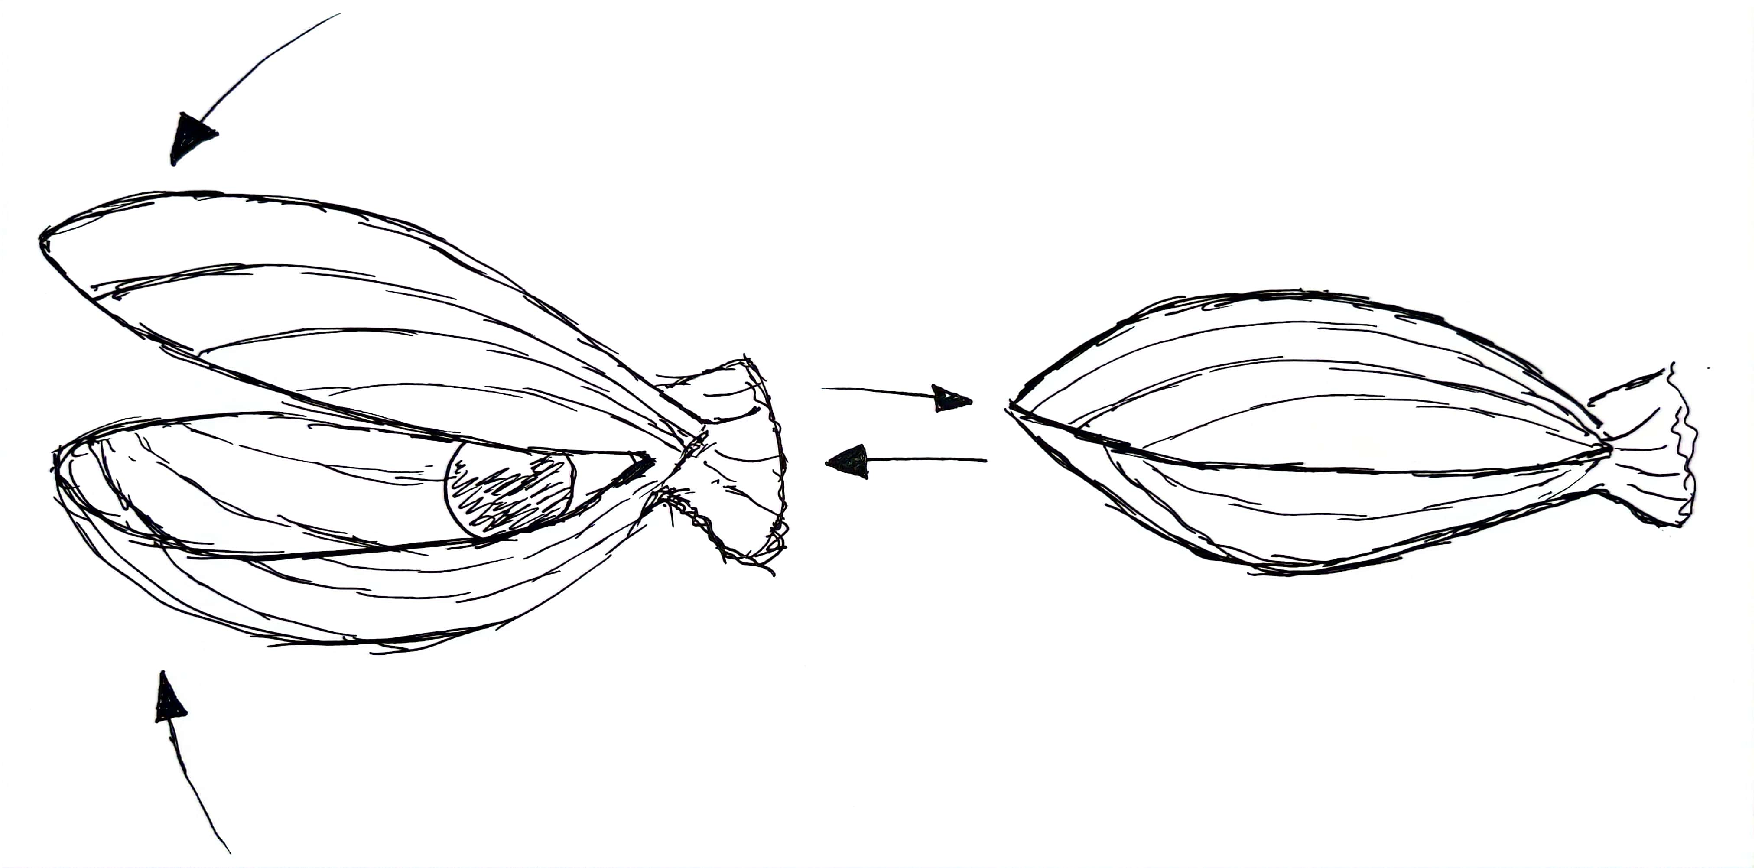
\includegraphics[width=.4\textwidth]{Figures/introduction/scallop.pdf}
    \caption{A scallop moves by opening and closing its shells, which in the Stokes regime gives zero net motion}
    \label{fig: scallop}
\end{figure}

The name comes from an example of reciprocal motion, a scallop opening and closing its shell.
A nonzero net self-propulsion therefore requires 
for the active particle to perform nonreciprocal cycles in configuration space.
\todo[noinline]{BM: we should add a schematics here.}
The solutions nature has found to overcome this problem include rotating a bundle of helical flagella, as is done by \textit{E. coli}, or using additional degrees of freedom allowing, e.g., to perform breast-stroke-like motion, as is done by \textit{Chlamydomonas}. 

%at least 2 independent degrees of freedom (d.o.f.) Examples of this are swimmers with a corkscrew flagella or breast-stroke-like motion.
Another consequence of the absence of inertia in the Stokes regime is that the swimmers cannot experience any net force or torque (the Stokes equation corresponding to a balance of momentum).
Hence, the force and torque generated by the flagella of the swimmers shown in Fig.~\ref{fig: swimmers} must be compensated by the drag their body exerts on the fluid\footnote{Assuming that the drag coming from the flagella can be neglected.}. 
In the far field, most microswimmers can thus be modeled as force and/or torque dipoles, whose nature will depend on how they locally actuate the fluid.\todo[noinline]{BM: Clear? Maybe need to rephrase in a better way...}

\begin{figure}[!htb]
    \centering
    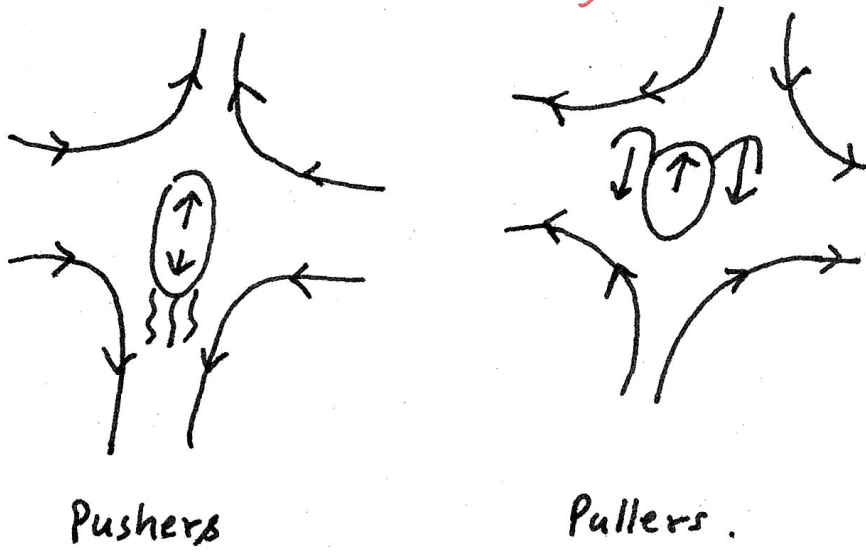
\includegraphics[width=.5\textwidth]{Figures/introduction/swimmers.png}
    \caption{Two examples of microswimmers showing the so-called \textit{pusher} and \textit{puller} configurations.}
    \label{fig: swimmers}
\end{figure}

We have seen that generating active motion at microscopic scales is far from being a simple task. The design and characterization of microscimmer self-propulsion mechanisms is in fact an active area of research. 
In chapter~\ref{chap_hydro}, we will discuss microswimmers hydrodynamics in more details.

% handwritten page VII

\section{A minimal model for active motion}
\label{intro_ABM}

In the previous section, we have discussed by which mechanism(s) active motion can arise in the context of microswimmers.
Here, we will ask a different question: what are the consequences of the presence of a self-propulsion speed on the dynamics of an active particle?
For this, we will model our swimmer/crawler/glider as an abstract `particle', and assume that it is able to sustain a finite self-propulsion velocity, but we won't be interested in the details of how this self-propulsion is realized.


\subsection{Some basics on Brownian motion}

\begin{figure}[!htb]
    \centering
    \includegraphics[width=.4\textwidth]{Figures/introduction/brownian.png}
    \caption{A Brownian particle is constantly interacting with the solvent molecules, resulting in an erratic motion.}
    \label{fig: brownian}
\end{figure}

Before discussing active motion, let us give a brief recap on the theory of the motion of Brownian (i.e., dead) particles.
Consider a micron-sized particle (e.g. a grain of polen, a colloid, etc..) in a fluid maintained at temperature $T$. 
The particle constantly undergoes collisions with the fluid molecules, and its mass is low enough so that these collisions result in an apparent erratic dynamics known as Brownian motion.
The dynamics of the particle can be modeled by the \emph{Langevin equation}
%
\begin{equation} \label{eq_LangevinBM}
    m\frac{\rmd^2 \bm r}{\rmd t^2} + \zeta \frac{\rmd \bm r}{\rmd t} = \bm f(t).
\end{equation}
%
Equation~\eqref{eq_LangevinBM} is nothing but Newton's second law, so that the first term on the left hand side represents the acceleration of the particle multiplied by its mass, and the second term accounts for the Stokes friction exerted by the fluid in response to the motion of the particle.
In fact, the ratio of the particle mass and friction coefficient defines a timescale $\tau = m / \zeta$ beyond which inertial effects can be neglected.
For a micron-sized sphere with a density comparable to that of water, we have
%
\begin{equation*}
    \tau = \frac{\rho \tfrac{4\pi}{3} R^3}{6 \pi \eta R} 
    = \frac{2\rho R^2}{9\eta} \approx 0.2 \; \mu{\rm s}.
\end{equation*}
%
For observation times beyond the micro-second, inertial effects can therefore be safely neglected. Hence, we will neglect the inertial term in~\eqref{eq_LangevinBM}, which we re-express in this overdamped limit as
\begin{equation} \label{eq_LangevinBM_ovd}
    \frac{\rmd \bm r}{\rmd t} = \frac{1}{\zeta}\bm f(t).
\end{equation}
%
The force term $\bm f$ is meant to model the random collisions that the particle undergoes with the solvent molecules, and is thus stochastic in nature.
Under the approximation that these collisions are isotropic, identically distributed and uncorrelated random events, we can use the central limit theorem to approximate the distribution of the stochastic process $\bm f$ by a normal distribution with zero mean and variance $\sigma^2$.
Namely, denoting averages with independent realizations of the noise with the notation $\langle \cdot \rangle$, the first two moments that fully characterize the distribution read
\begin{equation*}
    \langle f_i(t) \rangle = 0, \qquad
    \langle f_i(t) f_j(t') \rangle = \sigma^2 \delta_{ij}\delta(t - t').
\end{equation*}

Equation~\eqref{eq_LangevinBM_ovd} can be easily solved by integration, which leads to
\begin{equation*}
    \Delta \bm r(t) \equiv \bm r(t) - \bm r(t=0) = \frac{1}{\zeta} \int_0^t\rmd\tau \bm f(\tau).
\end{equation*}
Taking averages over the noise, this solution implies in particular that 
\begin{equation} \label{eq_BM_moments}
    \langle \Delta \bm r(t) \rangle = \bm 0, \qquad 
    \langle |\Delta \bm r(t)|^2 \rangle = d \sigma^2 t / \zeta^2,
\end{equation}
where $d$ is the number of spatial dimensions.
Equation~\eqref{eq_BM_moments} summarizes the two main features of Brownian (or diffusive) motion : it is associated with no net motion, and leads to a mean-squared displacement (MSD) linear in time.
The quantity $D = \sigma^2 / 2 \zeta^2$ corresponds to the diffusion coefficient of the particle.
Since both the viscous drag and stochastic force in~\eqref{eq_LangevinBM_ovd} originate from interactions between the particle and the solvent, the diffusion and friction coefficients are related by Einstein relation as $D = k_{\rm B}T / \zeta$.
This relation belongs to a more general class of equalities known as fluctuation-dissipation relations, and which are a hallmark of equilibrium (or near-equilibrium) dynamics.

\noindent
\textbf{Homework:} \textit{ By solving~\eqref{eq_LangevinBM} for the particle velocity $\bm v = \dd\bm r / \dd t$, show that the equipartition theorem imposes $\sigma^2 = 2 \zeta k_B T$. Deduce Einstein's relation from this result.
}

% Hand written page VIII

The problem of overdamped Brownian motion is sufficiently simple so that one can determine the full statistics of the particle displacement. 
For this, we define $\calP(\bm x,t) = \langle \delta(\bm x - \bm r(t)) \rangle$ as the distribution of the particle position, which obeys the Fokker-Planck equation\footnote{A simple way to demonstrate Eq.~\eqref{eq_FP_BM} is to take the time derivative of $\calP(\bm x,t) = \langle \delta(\bm x - \bm r(t)) \rangle$, and use Ito's lemma to expand the delta distribution.}
%
\begin{equation} \label{eq_FP_BM}
    \partial_t \calP(\bm x,t) - D \nabla^2 \calP(\bm x,t) = 0.
\end{equation}
%
Assuming that the particle sits at $\bm x = \bm 0$ at time $t=0$, the solution of Equation~\eqref{eq_FP_BM} is given by
\begin{equation*}
    \calP(\bm x,t) = \frac{1}{(4\pi D t)^{d/2}}e^{-\tfrac{|\bm x|^2}{4 D t}}.
\end{equation*}
We note that the mean of the distribution is at $\bm x = \bm 0$ at all times and that its width, i.e. the standard deviation, grows as $\sqrt{t}$ consistently with~\eqref{eq_BM_moments}.


\textit{
\noindent 
    {\bf Homework:} Consider a Brownian particle in a potential $U$, write the associated Fokker-Planck equation. Show that the stationary solution corresponds to the Boltzmann distribution.
For a harmonic potential $U = \tfrac{1}{2} k |\bm x|^2$, the time dependent solution of the FPE with initial condition $\calP(\bm x,0) = \delta(\bm x)$ is given by 
\begin{equation*}
    \calP(\bm x,t) = \left(\frac{\lambda}{2\pi D (1 - e^{-2\lambda t})}\right)^{d/2}e^{-\tfrac{\lambda}{2 D} \tfrac{|\bm x|^2}{1 - e^{-2\lambda t}}},
\end{equation*}
with $\lambda = k / \zeta$.
Calculate the mean and MSD associated with this distribution, comment.
}

\subsection{Active Brownian motion}

Although the previous section was devoted to the description of the dynamics of a passive particle, the Langevin equation~\eqref{eq_LangevinBM_ovd} does not assume that the particle is in an equilibrium state. 
Therefore, we can straightforwardly generalize to describe active motion it by assuming that the particle is able to self-generate a force leading to an active velocity $\va(t)$.  Equation~\eqref{eq_LangevinBM_ovd} now becomes
\begin{equation}\label{eq_LangevinABM}
    \frac{\rmd \bm r}{\rmd t} = \va(t) + \frac{1}{\zeta}\bm f(t).
\end{equation}
To fully characterize the dynamics, we now need to specify how $\va(t)$ evolves in time. 
As we have seen previously, self-propelled motion can arise in various ways, but what we argue below is that it most importantly introduces a finite persistence length in the dynamics.

To understand this, let us comment on real systems.
For example, the dynamics of bacteria like \textit{E. coli} consists of randomly alternating sequences of `run' and `tumble', respectively corresponding to straight motion along a fixed direction and random reorientations. 
Other active swimmers like self-propelled colloids, on the other hand, follow smooth trajectories as their self-propulsion direction slowly diffuses over time due to fluctuations.
In both cases, defining the typical particle velocity as $v_0$ and reorientation time $\tau_r$, we can build a persistence length by dimensional analysis as $\lp = v_0 \tau_r$.
Physically, on length scales below $\lp$ the active particle exhibits ballistic motion along a fixed direction with a speed $\approx v_0$, while on scales $\gg \lp$ its direction of motion has randomized so that its overall dynamics is isotropic and diffusive. 


\begin{figure}[!htb]
    \centering
    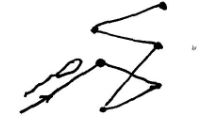
\includegraphics[width=.25\textwidth]{Figures/introduction/runandtumble.png}
    \hspace{2cm}
    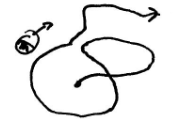
\includegraphics[width=.2\textwidth]{Figures/introduction/smooth.png}
    \caption{Run and tumble versus smooth active trajectories resulting from different modes of self-propulsion.}
    \label{fig: run and tumble vs smooth}
\end{figure}

As a minimal model of active velocity, we can thus simply assume that the particle self-propels at constant speed $v_0$, while the unit vector $\he$ parametrizing its orientation is a colored noise with zero mean and exponential correlations:
\begin{equation} \label{eq_cf_e}
    \langle \he(t) \cdot \he(t + \tau) \rangle = e^{-\tau / \tau_r}.
\end{equation}

\textit{
\noindent 
    {\bf Homework:} 
    Consider an active particle moving in two dimensions,
    so that its self-propulsion direction is parametrized by a single angle $\theta(t)$.
    \begin{enumerate}
        \item Modeling tumbles as isotropic and uncorrelated random events occurring with a rate $\lambda$, show that the associated probability distribution is given by
        \begin{equation*}
            P(\theta,t) = e^{-\lambda t}\delta(\theta) + \frac{1}{2\pi}\left(1 - e^{-\lambda t} \right).
        \end{equation*}
        Here, we have assumed for simplicity that $\theta = 0$ at time $t = 0$.
        \item In the case where $\theta$ diffuses in time with a diffusion coefficient $D_r$, show that the associated distribution is a Gaussian with zero mean and variance $2 D_r t$.
        \item For both cases 1. and 2. deduce that the 
        particle self-propulsion direction satisfies $\E{\hat{\bm e}(\theta(0))\cdot \hat{\bm e}(\theta(\tau))} = \exp(-\tau/\tau_r)$, and express $\tau_r$ as a function of $D_r$ and $\lambda$.
    \end{enumerate}
    }


We immediately deduce from~\eqref{eq_cf_e} that, under the assumption that the active and Brownian noises are independent,
\begin{align}
    \langle |\Delta \bm r(t)|^2 \rangle & = 2 d D t 
    + v_0^2 \int_0^t\rmd\tau_1\int_0^t\rmd\tau_2 \, e^{-|\tau_1-\tau_2|/\tau_r} \nonumber \\
    & = 2 d D t 
    + 2 \lp^2 \left( \frac{t}{\tau_r} - 1 + e^{-t/\tau_r} \right).
\end{align}
%
This expression can be simplified by considering the limiting regimes $t \gg \tau_r$ and $t \ll \tau_r$,
which respectively give
%
\begin{align*}
    \langle |\Delta \bm r(t)|^2 \rangle & 
    \underset{t \ll \tau_r}{\simeq} 2 d D t + v_0^2 t^2 , \\
    \langle |\Delta \bm r(t)|^2 \rangle & 
    \underset{t \gg \tau_r}{\simeq} 2 d D_{\rm eff} t , \qquad  D_{\rm eff} = D + \frac{v_0^2\tau_r}{d}. 
\end{align*}
%
The active particle MSD therefore highlight three dynamical regimes shown in Fig.~\ref{fig: MSD}:
\begin{itemize}
    \item Thermal diffusion dominates at short times ($t \ll 2 d D / v_0^2)$.
    \item At intermediate times ($2 d D / v_0^2 \ll t \ll \tau_r)$, activity contributes and motion is ballistic with a typical speed $v_0$.
    \item At long times ($t \gg \tau_r$) the self-propulsion direction has randomized, resulting in a diffusive motion with an enhanced diffusion coefficient.
\end{itemize} 

Due to the finite correlation time of its self-propulsion orientation, the long-time dynamics of an active particle is therefore ``Brownian-like'' (i.e. diffusive).
However, the associated effective diffusion coefficient $D_{\rm eff}$ does not satisfy the fluctuation-dissipation relation, which is a clear signature that the dynamics is out-of-equilibrium.

\begin{figure}[!htb]
    \centering
    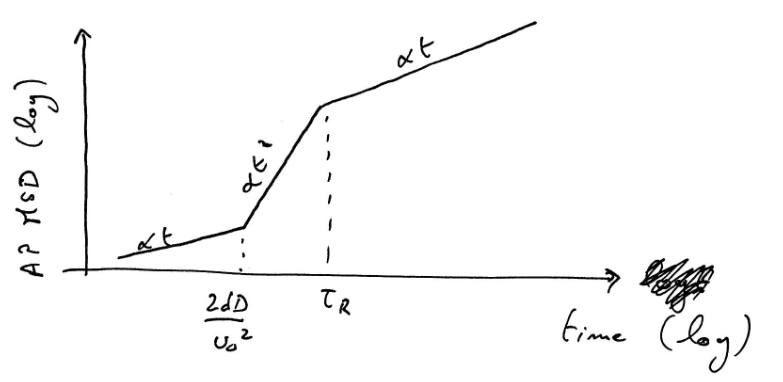
\includegraphics[width=.6\textwidth]{Figures/introduction/crossover.png}
    \caption{The mean-square displacement of an active Brownian particle showing the three dynamical regimes discussed in the main text.}
    \label{fig: MSD}
\end{figure}



% Handwritten page XIII

\section{Phase transitions and critical phenomena}

The concept of phase transition plays a central role in the study of active systems.
A prominent example the emergence of flocking behavior which we will study in more details in Chapter~\ref{chap_polar}, where directed units spontaneously choose a direction to align in and move together as a flock.
This phenomenon can be conceptually interpreted as a nonequilibrium phase transition, where rotational symmetry is spontaneously broken.
In some sense, flocks thus correspond to an active version of ferromagnetic materials, where spins do not sit on the sites of a lattice but can freely move.
%This is the Active Matter version of the ordering transition in the Ising model, in which spins align in the case of a ferromagnet or anti-align in the case of an anti-ferromagnet.
In this section, we will review some of the basic features of the theories of phase transitions at equilibrium, and introduce tools that will be useful in the context of active matter.



\subsection{A simple example: the Ising model}

One of these important features of phase transitions is that they are associated with the notion of scale-invariance.
The simplest illustration of this can be obtained by analyzing the Ising model.
We consider $N$ spins, $s_i = \pm 1$ on a lattice, and define an energy function as
%
\begin{align} \label{eq_energy_Ising}
    E = - \frac{J}{2} \sum_{\E{ij}} s_i s_j.
\end{align}
%  
Here, $\E{ij}$ indicates that the sum is over all pairs of neighbors $(i,j)$ on the lattice, while the factor $\tfrac{1}{2}$ prevents double counting. 
For $J > 0$, minimizing $E$ will thus favour configurations for which neighbouring spins are aligned, while if $J < 0$ they will preferably anti-align.
The equilibrium state of the model is captured by the partition function, which in the canonical ensemble is obtained by summing the Boltzmann weights associated with all possible spin configurations $\{s_i\}$:
%
\begin{align}
    Z = \sum_{\{s_i\}} e^{-\beta E},
\end{align}
%
where $\beta = (k_B T)^{-1}$.
To measure the amount of order in the system, we also define the order parameter,
%
\begin{align}
    m = \frac{1}{N}\sum_i s_i,
\end{align}
%
which is usually called the magnetization.
If all spins points along the same direction $|m|  = 1$, while if they completely disordered $m \to 0$.

To get a qualitative understanding of the phenomenology of the model, we use a simple mean-field analysis and assume that each spin weakly fluctuates around its mean value $m$, so that we write $s_i \approx m + \delta s_i$, with $\delta s_i$ small.
Then, at linear order in the perturbation,
%
\begin{align*}
    s_i  s_j = m^2 + m(\delta s_i + \delta s_j) + \Oh(\delta s^2)
    \approx m(s_i + s_j - m).
\end{align*}
%
%Here, we have neglected terms that are second order in the perturbations $\delta s$.
% Handwritten page XIV
Under this assumption, we rewrite the total energy~\eqref{eq_energy_Ising} as
%
\begin{align*}
    E_{\rm MF} 
    &= \frac{1}{2} J m \sum_{\E{ij}}(m - s_i - s_j)
    = \frac{1}{2} J m z \left(m N - 2 \sum_{i} s_i  \right).
\end{align*}
%
Here, $z$ is the number of nearest neighbors for each site, i.e. the coordination number of the lattice.
Its value depends on the structure of the lattice and the dimensionality of space.
For square and cubic lattices, $z = 2 d$, where $d$ is the dimension of space.
At the mean field level, the partition function therefore reads
%
\begin{align}
    Z_{\rm MF} & = \sum_{\{s_i\}} \exp \left\{\frac{1}{2}\beta J m z \left( 2\sum_{i} s_i - mN \right) \right\} \nonumber \\
    & = e^{-\frac{1}{2}\beta J z N m^2} 
    \sum_{\{s_i\}} \prod_{i} e^{\beta J m z s_i} \nonumber \\
    & = e^{-\frac{1}{2}\beta J z N m^2} 
    \left[\sum_{s = \pm 1} \exp \left(\beta J m z s \right)\right]^N \nonumber\\
    & = e^{-\frac{1}{2}\beta J z N m^2} \left[2 \cosh \beta J m z\right]^N, \nonumber
\end{align}
%
The Helmholtz free energy of the system is obtained by taking the logarithm of the partition function, $\beta F = - \ln Z$, so that
%
\begin{align} \label{eq_Ising_FMF}
    \beta F_{\rm MF} = N \left[ \frac{1}{2}\beta Jm^2 z - \ln\left(\cosh \beta J m z\right) \right],
\end{align}
%
where we have discarded irrelevant constant contributions.
At constant volume and temperature,  the equilibrium state of the system minimizes the total free energy.
The magnetization of the system is therefore obtained from 
%
\begin{align} \label{eq_Ising_mMF}
    \pdv{F_{
    \rm MF}}{m} = 0
    \iff m = \tanh (\beta J m z).
\end{align}
%
Equation~\eqref{eq_Ising_mMF} can be solved graphically by drawing both its l.h.s.\ and r.h.s.\ as a function of $m$, as illustrated in Fig.~\ref{fig: The graphical solution of the mean field free energy minimization.}.
In particular, we note that the $\tanh(\beta J m z)$ function is strictly monotonous in $[-1;1]$, while its maximum slope at $m=0$ is given by $\beta J z$. 
Therefore, when $\beta J z < 1$ the only solution of~\eqref{eq_Ising_mMF} corresponds to $m = 0$,
while for $\beta J z > 1$ a pair of additional solutions $m = \pm m_0 \ne 0$ emerges.
Taking the second derivative of $F_{\rm MF}$, one can also show that for $\beta J z > 1$ the solutions $m = \pm m_0$ correspond to two degenerate minima, while $m = 0$ is a local maximum.

\begin{figure}[!t]
    \centering
    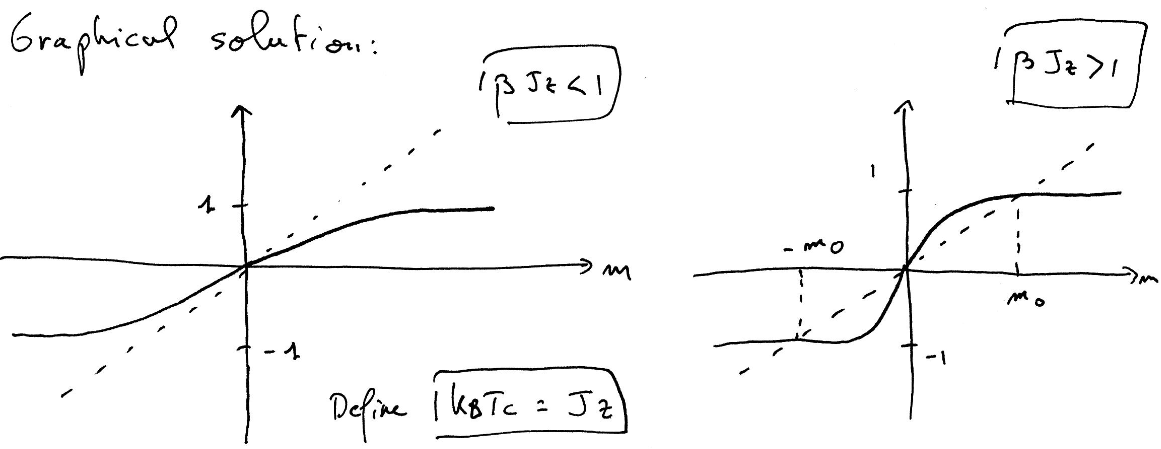
\includegraphics[width=\textwidth]{chapters/Figures/introduction/minimize.png}
    \caption{Minimization for different cases}
    \label{fig: The graphical solution of the mean field free energy minimization.}
\end{figure}

Hence, there exists is finite value of the system temperature $k_B T_c = J z$ that marks a qualitative change in the equilibrium properties of the system.
This is exactly the definition of a phase transition, which is here associated to the emergence of a macroscopic magnetization in the system. 
% This shows that for inverse temperatures $\beta = 1 / k_B T$ so that $\beta J z < 1$, there is only one stationary point free energy, $m = 0$.
% In this case, this is also a minimum.
% For $\beta J z > 1$, there appear two additional stationary $m = \pm m_0$ points.
%These are now two degenerate minima of the free energy, while $m = 0$ is a local maximum.
%There is thus a \emph{phase transition} at the finite, critical temperature defined by $k_B T_c = J z$.
For $T \le T_c$, the $m \rightarrow - m$ symmetry of the theory is spontaneously broken, as the magnetization $m$ randomly settles at one of the degenerate minima $\pm m_0$.
If we now study the behavior of the system close to the transition, we can assume that $m$ is small and expand the free energy around $T \approx T_c$
so as to obtain a simplified expression known as the \textit{Landau free energy}:
%
\begin{align} \label{eq_LandauFE_Ising}
    F_{\rm MF}
    \underset{T \to T_c}{\simeq} 
    \frac{1}{2} Nk_B T_c
    \left( \vartheta m^2 + \frac{m^4}{6}\right)
    + \Oh(m^6),
\end{align}
%
where we have defined the reduced temperature $\vartheta \equiv (T - T_c) / T_c$, often called the control parameter. 

Thanks to its simple form, it is easier to get an intuitive picture from~\eqref{eq_LandauFE_Ising} of the changes in the free energy landscape that induce the phase transition.
%t has the form $F = \frac{1}{2} \alpha t m^2 + \beta \frac{1}{4} m^4$.
As $\vartheta$ changes sign, the free energy transitions from a single-well to a double-well structure with two degenerate minima.
This feature is very general, so that using symmetry arguments one can always write the free energy of the system in the form of~\eqref{eq_LandauFE_Ising}, regardless of the details of the microscopic dynamics.
This points out to the existence of a kind of universality in the properties of the system close to the ordering transition, but to understand it fully we now need to account as well for the spatial dynamics of $m$.

\begin{figure}[!t]
    \centering
    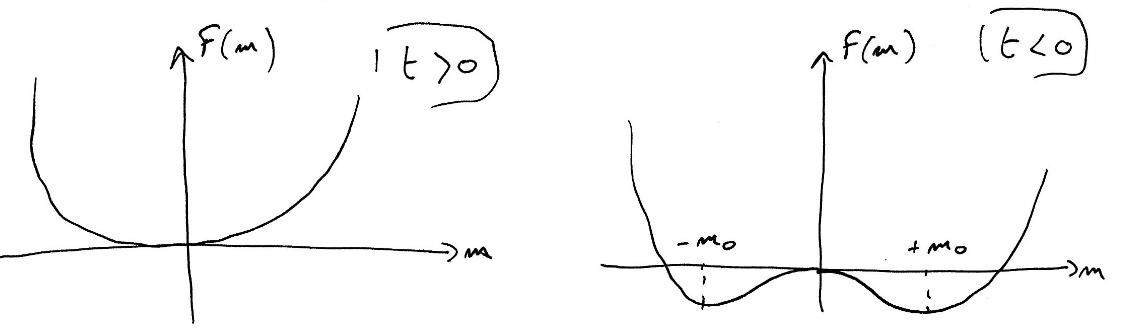
\includegraphics[width=.8\textwidth]{chapters/Figures/introduction/double_well.png}
    \caption{The double Landau free energy changes from a single to a double well as the control parameter is tuned past the critical point.}
    \label{fig: double well}
\end{figure}

%To go beyond the mean-field approach, we include spatial dynamics.
From now, the system magnetization will thus no more be a simple number, but a field that depends on space and time $m = m(\bm x,t)$.
Considering a small subvolume of the system $\rmd\bm x$, close enough to the transition we can thus reasonably assume that the associated `bulk' free energy is given by $f(m) \rmd\bm x$
with
%
\begin{align}
    f(m) = \frac{1}{2}\alpha \vartheta  m^2 + \frac{1}{4} \beta m^4,
\end{align}
%
where $\alpha \approx k_B T_c$ and $\beta \approx k_B T_c / 3 \approx \alpha / 3 $. 
Of course, we also need to account for the fact that $m$ cannot change arbitrarily fast between neighboring subvolumes, so that the presence of finite gradients must come at a cost.
%This is the ``Bulk free energy density''.
%The full free energy is the integral of this density, plus a term that takes into account the cost of gradients.
The simplest way to do this while preserving the invariance of the free energy under $m \to -m$ and rotations of space (which must always be obeyed as they are symmetries of the microscopic dynamics) is to include a term $\propto |\nabla m|^2$ in the free energy density.
Combining these terms together gives us the Ginzburg-Landau free energy functional\footnote{\emph{Functional}, not function, as $F[m]$ is a function of a function $m(\bm x)$. 
This means that the minimum of $F[m]$ is not determined by using derivatives $\odv{}{m}$, but functional derivatives $\fdv{}{m(\bm x)}$.}
%
\begin{align} \label{eq_GL_Ising}
    F[m] = \int \dd \bm x 
    \left(f(m) + \frac{1}{2} K |\nabla m|^2\right).
\end{align}
%

Analogously to the mean field analysis, the equilibrium magnetization profile minimizes the free energy~\eqref{eq_GL_Ising}. 
Namely, the associated condition is
$\delta F / \delta m(\bm x) = 0$, where the $\delta$ symbol indicates that we perform a functional derivative.
In fact, here we won't really be interested in the mean magnetization profile, but rather in characterizing the behaviour of the fluctuations around it.
One way to achieve this is to generalize the Langevin approach that we used in Sec.~\ref{intro_ABM} to model the dynamics of fields.
Namely, under the reasonable assumption that the force acting on $m$ derives from the free energy functional, we can write\footnote{We will see in Chapter~\ref{chap_thermo} how this form of the equation of motion gives the correct detailed-balance condition on the stochastic field dynamics.}
%To obtain a dynamical equation for this system, which governs the time-evolution of $m$, we assume purely dissipative dynamics, 
%
\begin{align} \label{eq_dyn_m_Ising}
    \partial_t m(\bm x, t)
    =
    - \fdv{F}{{m(\bm x, t)}} + \psi(\bm x,t)
    = - [\alpha \vartheta + \beta m^2(\bm x, t)] m(\bm x, t) + K \nabla^2 m + \psi(\bm x,t),
\end{align}
%
where $\psi$ is Gaussian white noise satisfying
%
\begin{align*}
    \E{\psi(\bm x, t)} &= 0, &
    \E{\psi(\bm x, t) \psi(\bm x', t')}
    = \Psi \delta(\bm x - \bm x') \delta(t - t').
\end{align*} 

Momentarily discarding the noise, Eq.~\eqref{eq_dyn_m_Ising} admits a homogeneous steady state solution $m_0$ given by
%
\begin{align*}
    (\alpha \vartheta + \beta m_0^2) m_0 = 0
    \implies
    \begin{cases}
        m_0 = 0, & \vartheta > 0, \\
        m_0 = \sqrt{ \frac{ \alpha |\vartheta| }{ \beta } }, & \vartheta \le 0,
    \end{cases}
\end{align*}
%
consistently with our previous analysis.
To study how this homogeneous solution is affected by the presence of fluctuations, we now write the magnetization field as $m(\bm x, t) = m_0 + \delta m(\bm x, t)$ and study the dynamics of $\delta m$ at the linear level.
The perturbation obeys the equation of motion
%
\begin{align} \label{eq_dm_Ising}
    \partial_t \delta m = - a^2 \delta m  + K \nabla^2 \delta m + \psi,
\end{align}
%
where the damping rate
%
\begin{align*}
    a^2 \equiv 
    \begin{cases}
        \alpha \vartheta, & \vartheta > 0, \\
        2 \alpha |\vartheta|, & \vartheta \le 0,
    \end{cases}
\end{align*}
%
is positive in both phases.
Because it is linear, Equation~\eqref{eq_dm_Ising} is easily solved in Fourier space, so that we define for any field $\phi(\bm x,t)$
%
\begin{align*}
    \hat \phi(\bm q, \omega)
    =
    \int \dd \bm x \dd t \, e^{i(\bm q \cdot \bm x + \omega t)} \phi(\bm x, t), \qquad
    \phi(\bm x, t)
    =
    \int \frac{\dd \bm q \dd \omega}{(2\pi)^{d+1}} \, e^{-i(\bm q \cdot \bm x + \omega t)}
    \hat \phi(\bm q, \omega).
\end{align*}
%
We then get
%
\begin{align}
    (i \omega + a^2 + Kq^2)\delta \hat m(\bm q,\omega) = \hat \psi(\bm q, \omega),
\end{align}
%
where $q = |\bm q|$ and the Fourier transform of the noise keeps a vanishing expectation value and has a covariance
%
\begin{align*}
    \E{\hat \psi(\bm q, \omega)\hat\psi(\bm q', \bm \omega')}
    = \Psi (2\pi)^{d + 1}\delta(\bm q + \bm q') \delta(\omega + \omega').
\end{align*}
%
With this, we easily can explicitly calculate the Fourier transform of the two-point correlation function,
%
\begin{align*}
    \hat C(\bm q, \bm \omega)
    = 
    \frac{\E{\delta \hat m(\bm q, \omega) \delta \hat m(-\bm q, -\omega)}}{(2\pi)^{d + 1}\delta(\bm q + \bm q') \delta(\omega + \omega')  }
    = 
    \frac{\Psi}{\omega^2 + (a^2 + K q^2)^2}.
\end{align*}
%
We obtain the equal-time correlation by integrating over all frequencies. Performing the integral\footnote{Using that 
$\int_{-\infty}^{+\infty} \tfrac{\dd x}{2\pi} \tfrac{1}{x^2 + a^2} = 
\tfrac{1}{2\pi a}\int_{-\infty}^{+\infty} \tfrac{\dd y}{y^2 + 1} = \tfrac{1}{2\pi a} [\arctan(y)]_{-\infty}^{+\infty}= \tfrac{1}{2a}$}, 
we get
%by contour integration 
\todo[noinline]{Draw contour, explain
BM: Not necessary, one can simply express the indefinite integral in terms of arctan.}
%
\begin{align}
    \hat C(\bm q) \equiv \int_{-\infty}^{+\infty} \frac{\dd \omega}{2 \pi} \hat C(\bm q, \omega)
    = 
    \frac{1}{2}\frac{\Psi }{a^2 + K q^2}.
\end{align}
%
The real space two-point correlation function is then
%
\begin{align}
    C(\bm x)
    = \E{\delta m(\bm 0) \delta m(\bm x)}
    & = \frac{\Psi}{2 K}
    \int \frac{\dd \bm q}{(2 \pi)^d} \frac{e^{-i\bm q \cdot \bm x}}{\xi^{-2} + q^2}, \nonumber \\
    \label{eq_CF_Ising}
    & = \frac{\Psi}{2 K}
    \int \frac{\dd q}{2 \pi} 
     \frac{q^{d-1}}{\xi^{-2} + q^2}
    I(q x),
    %\int \frac{\dd\Omega}{(2\pi)^{d-1}}   \frac{e^{-i q x \cos\theta}}{\xi^{-2} + q^2}, \nonumber \\
\end{align}
%
where we have introduced the \emph{correlation length}
%
\begin{align} \label{eq_corr_length}
    \xi \equiv \sqrt{ \frac{ K }{ a^2 } },
\end{align}
%
while $I(q x) = \int \tfrac{\dd\Omega_q}{(2\pi)^{d-1}} \exp(- i \bm q \cdot \bm x)$, and the integration is performed over all orientations of $\bm q$.
As expected from the symmetries of the problem, the correlation function $C(x)$ is isotropic, and measures how much, on average, fluctuations in the magnetization are correlated over a distance $x$. 
The correlation length $\xi$ basically measures the length scale over which these correlations are significant.
We may see this by taking the two limits of the integral~\eqref{eq_CF_Ising}
%
\begin{align*}
    C(x) \simeq
    \begin{cases}
        x^{2-d} & x \ll \xi, \\
        x^{1-d/2} e^{- x / \xi} & x \gg \xi.
    \end{cases}
\end{align*}
%
Therefore, over distances less than the correlation length, the correlations exhibit a slow algebraic decay, $C(x) \sim x^{2 - d}$, while over distances much larger than $\xi$ they are exponentially suppressed.

As $\xi \propto 1/\sqrt{ |\vartheta| }$ (see Eq.~\eqref{eq_corr_length}), the correlation length is finite in both the disordered and ordered phases.
On the other hand, when approaching the transition $\vartheta \to 0$ the correlation length diverges, and the correlations become \emph{scale free}.
$\vartheta = 0$ defines a \emph{critical point}, which corresponds to a parameter regime where the dynamics of fluctuations has no intrinsic length scale, which can be visualized directly \href{https://www.youtube.com/watch?v=lQxD1PinDbs}{from simulations}.

Another consequence of the divergence of $\xi$ is that the large scale physics at the critical point is independent of the microscopic details of the model.
This property is at the root of the powerful concept of \emph{universality} commonly used in condensed matter physics.
At a critical point, the only features that govern the relevant large scale physics are fundamental characteristics of a system like its symmetries, the conservation laws it obeys, and its dimensionality.
Systems sharing the same characteristics are said to belong to the same universality class, and are thus formally described by the same theory.

A critical point is characterized by a set of critical exponents, which describe how various observables behave in its vicinity.
Examples we have already met include
%
\begin{align}
    |m_0| &\sim |\vartheta|^\beta, &
    \xi & \sim |\vartheta|^{-\nu}, &
    C(x) & \sim x^{d - 2 + \eta},
\end{align}
%
with the mean field exponents $\beta = \nu = \tfrac{1}{2}$ and $\eta = 0$.
To obtain these values we have assumed that the typical fluctuations of $m$ around its mean $m_0$ are small, so that we obtained a linear equation for the perturbations.
As the critical point corresponds to the vanishing of the damping term in Eq.~\eqref{eq_dm_Ising}, 
we can however reasonably question the validity of this approximation.
%these mean field predictions are generally incorrect, because we have neglected the non-linearities in the equation, and we have not taken into account the effects of fluctuations.

In fact, the Ising model can be solved exactly in dimensions one and two, 
and the corresponding solutions (unsurprisingly) do not match the predictions of the mean field theory.
Namely, in one dimension the dynamics is dominated by entropy: spins have too few nearest neighbors to for the alignment to compete with fluctuations, so that the system is disordered at any finite temperature.
In two dimensions, the mean field calculation only gives a qualitatively correct picture. 
The exact solution derived by Onsager indeed predicts the existence of a critical point at a finite $T_c$, but the exact exponents are different from their mean field values.  
A similar situation is found in three dimensions, although the absence of an exact solution imposes to determine the exponents numerically.
In the end, the mean field theory is only quantitatively valid in dimensions higher than $4$, while $d_c = 4$ is known has the upper critical dimension of the model.
The values of the critical exponents in $d \ge 2$ are reported in Table~\ref{table_Ising_exp}.

A refined prediction for the value of the exponents in three dimensions requires to take into account the effect of nonlinearities, which can be done using the theoretical framework of the \emph{Renormalization Group} (RG).
%In fact, the one-dimensional Ising model can be solved exactly, and \emph{does not} feature a phase transition at finite temperature. In one dimension, there are too few nearest neighbors to keep spins ordered when thermal noise is introduced, and any non-zero temperature results in a finite correlation length.
%In the case of the Ising model, the mean-field breaks down for all dimensions lower than its \emph{critical dimension}, $d < d_c = 4$.
%To go beyond the mean field prediction and obtain accurate results for the critical exponents, one has to employ the \emph{Renormalization Group} or RG for short.
The RG framework relies on the scale invariance property of the critical point.
Its main idea is to study how the parameters of the free energy~\eqref{eq_GL_Ising} ($\alpha$, $\beta$ and $K$) renormalize as one changes the scale of the theory and integrates out the short wavelength physics. 
This approach leads to equations whose solution tell us how the effective parameters of the theory `flow' as we investigate the physics over larger and larger scales. 
The critical point then corresponds to a fixed point of these equations, meaning that the parameters do not change anymore with the scale of the theory: the physics is scale-free.
You can find a visual illustration of these ideas \href{https://www.youtube.com/watch?v=MxRddFrEnPc}{here}.
\todo[inline]{BM: Is this clear (wanted to stay brief)? Could we maybe show a sketch of a flow diagram as an illustration?}
For a more detailed introduction on RG, we invite you to read textbook references~\cite{Goldenfeld1992,Kardar2007}. 

%In this method, one explicitly integrates out the short-wavelength dynamics.
%With this, one may derive equations describing how the parameters in the free energy, such as $\alpha$ and $\beta$ above, change as one changes the scale of the theory.
%These are the \emph{Renormalizatio Group Equations}.
%A fixed point in the RG equations means that the parameters do not change, and thus that the corresponding model is scale-free.
%Below we report some of the exponents for the Ising model.


%In 3 dimensions, one has to resort to renormalization or numerics.
%In the table below, we provide some the exponents in various dimensions.
%Those in 2D are exact, the 3D ones are from numerics, while those above 4D are the mean-field exponents.

\begin{table}[h]
    \centering
    \caption{Critical exponents of the Ising model. Those in $d=2$ are exact, the $d=3$ ones are obtained from numerical simulations~\cite{CampostriniPRE2002}, while those in $d \ge 4$ are follow from the mean field analysis.}
    \begin{tabular}{r|c c c}
        $d$ & 2 & 3 & $\ge 4$ \\
        \hline
        $\beta$ & $1/8$ & $0.32653(10)$ & $1 / 2$ \\
        $\nu$ & $1$ & $0.63012(16)$ & $1 / 2$ \\
        $\eta$ & $1/4$ & $0.03639(15)$ & $0$
    \end{tabular}   
    \label{table_Ising_exp}
\end{table}


\subsection{Continuous symmetries: Goldstone modes and the Mermin-Wagner theorem}

At the beginning of this section, we motivated the present introduction on critical phenomena by mentioning the example of flocking.
Contrary to Ising spins which can only take discrete values, birds are free to move in any direction they please.
Hence, the self-propulsion direction of a bird is better described by a vector than a scalar.
Here, we will therefore stay within the framework of equilibrium systems, but make a step closer to actual birds by extending our analysis to systems presenting a continuous rotational symmetry.

%The Ising model has the discrete symmetry $s_i \rightarrow -s_i$, in mathematical terms $\mathbb{Z}_2$.
%The equations of motion, and thus all physics, remain unchanged if all spins are flipped upside-down.
%We will now consider spins that are free to rotate around, and not just point up or down so that the spin at each site is represented by a vector $\bm s_i$.

We therefore consider $N$ vector spins $\{\bm s_i\}$, each having $n$ components, on a lattice in $d$ dimensions.
The magnetization measuring the amount of order in the system is thus also a vector, 
%
\begin{align}
    \bm m = \frac{ 1 }{ N } \E{{\sum}_i \bm s_i},
\end{align}
%
while the energy function~\eqref{eq_energy_Ising} is generalized to
%
\begin{align} \label{eq_energy_ON}
    E = - \frac{J}{2} \sum_{\E{ij}} \bm s_i \cdot \bm s_j.
\end{align}
%
By construction, the energy~\eqref{eq_energy_ON} remains unchanged when one rotates all spins at the same time.
This class of transformations belongs to the orthogonal symmetry group $\mathrm{O}(n)$, so that the model defined by~\eqref{eq_energy_ON} is usually referred to as the $\mathrm{O}(n)$ model.
Note that the Ising model we studied previously corresponds to the particular case $n = 1$ (in this case the symmetry is of course discrete and amounts to flipping all spins),
while the $n = 2$ and $n = 3$ are respectively known as the $XY$ and Heisenberg models.

%This symmetry, which in group theory is called a $\mathrm{O}(n)$ symmetry where $n$ is the number of dimensions of the vector being rotated, is continuous.

We now generalize the Ginzburg-Landau approach presented in the previous section to this case with continuous symmetries.
Assuming again a regime where the amplitude of the vector $\bm m$ is small, we write a low-order expansion of the free energy that satisfies the $\mathrm{O}(n)$ symmetry:\footnote{
For simplicity, we have set $\alpha = \beta = 1$. This choice of parameters basically amounts to a specific choice of units for $\vartheta$ and $|\bm m|$.}
%
\begin{align} \label{eq_FE_ON}
    F = \int \dd \bm x \, 
    \left(
        \frac{\vartheta}{2}  |\bm m|^2 + \frac{1}{4} |\bm m|^4 + \frac{K}{2} |\nabla \bm m|^2
    \right),
\end{align}
%
where the gradient term should be understood as $|\nabla \bm m|^2 = \sum_{i, \alpha}\nabla_i m_\alpha \nabla_i m_\alpha$.
For $\vartheta > 0$, the bulk part of the free energy~\eqref{eq_FE_ON} corresponds to a single well centered at $\bm m = \bm 0$, while for $\vartheta < 0$ it has a continuum of degenerate minima satisfying $|\bm m| = \sqrt{|\vartheta|}$.
For $n = 2$, in particular, the free energy landscape takes the well-known Mexican-hat shape shown in Fig.~\ref{fig: mexican}.

\begin{figure}[!t]
    \centering
    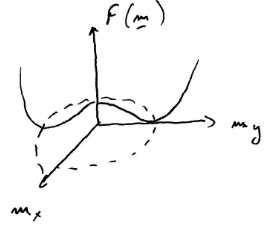
\includegraphics[width=.6\textwidth]{chapters/Figures/introduction/mexican.png}
    \caption{The Mexican-hat potential.}
    \label{fig: mexican}
\end{figure}

%Here, the gradient term represents a dot-product of both the gradients and the magnetization, $|\nabla m|^2 = \nabla_\alpha m_\beta \nabla_\alpha m_\beta$.
We now follow the same procedure as before, leading to the stochastic dynamics,
%
\begin{align}
    \partial_t \bm m = - (\vartheta + |\bm m|^2) \bm m + K \nabla^2 \bm m
    + \bm \psi,
\end{align}
where the noise $\bm \psi$ has zero mean and correlations
\begin{align*}
    \E{\psi_i(\bm x, t) \psi_j(\bm x', t')}
    = \Psi \delta_{ij} \delta^d(\bm x - \bm x') \delta(t - t') 
    \qquad \forall i,j \in [0;n].
\end{align*} 
%

As before, the steady-state solution of the deterministic equation
%
\begin{align*}
    |\bm m_0|^2 
    =
    \begin{cases}
        0, & \vartheta > 0 \\
        |\vartheta|, & \vartheta < 0 
    \end{cases}
\end{align*}
%
only defines the magnitude of the mean order, while its direction remains arbitrary and is picked at random by the system.
%Now, the steady-state solution is picked not from two degenerate minima, but instead from a continuum of degenerate minima.
We thus write the deterministic stationary solution as $\bm m_0 = m_0 \hat {\bm u}_\parallel$, where $\hat {\bm u}_\parallel$ is a $n$-dimensional unit vector giving the direction of the 
mean order.
We also expand $\bm m$ in terms of longitudinal and transverse perturbations
%
\begin{align*}
    \bm m &= (m_0 + \delta m_\parallel) \hat {\bm u}_\parallel + \delta \bm m_\perp,
\end{align*}
%
such that $\delta \bm m_\perp \cdot \hat {\bm u}_\parallel = 0$.
You can easily convince yourself that the analysis of the disordered phase $\vartheta > 0$ will not lead to any qualitatively new behavior w.r.t. what we have discussed for the Ising model, so here we will focus on analysing the ordered solution, i.e., taking $\vartheta < 0$.
The linearized equations for the perturbations are then
%
\begin{subequations}
\begin{align}
    \label{eq_ON_dmpara}
    \partial_t \delta m_\parallel 
    & = 
    2 t \delta m_\parallel + K \nabla^2 \delta m_\parallel + \psi_\parallel, \\
    \label{eq_ON_dmperp}
    \partial_t \delta \bm m_\perp
    & = K \nabla^2 \delta \bm m_\perp + \bm \psi_\perp,
\end{align}
\end{subequations}
%
where $\psi_\|$ and $\bm \psi_\perp$ correspond to projections of the noise along the longitudinal and transverse directions, and remain uncorrelated Gaussian white noises with variance $\Psi$.

Comparing Eqs.~\eqref{eq_dm_Ising} and~\eqref{eq_ON_dmpara},
it is clear that the longitudinal fluctuations are described by the same equation as for the Ising model, so that they are correlated over a finite correlation length $\xi_\| = \sqrt{ K / 2 |\vartheta| }$.
The dynamics of transverse perturbations, on the other hand, is not damped so that it is
associated with a diverging correlation length for all $\vartheta \le 0$.
The reason for this is quite intuitive: a uniform transverse perturbation $\delta\bm m_\perp$ corresponds to a global rotation of the mean order, which comes at zero energetic cost. 
Depending on who you are talking to, $\delta \bm m_\perp$ will be called a \emph{Goldstone mode}, a \emph{spin wave} or,
in the language of high-energy physics, a \emph{massless mode}.
%This results from the spontaneous breaking of a continuous symmetry. When this happens, there is no energetic cost associated with a global rotation. Consider the Mexican hat, given some direction of symmetry breaking, one can always rotate the corresponding unit vector around the center without incurring an energetic cost.

Goldstone modes are associated with the presence of a continuous symmetry, and their presence has important consequences.
First, the spatial correlations of the order parameter are scale-free:
%
\begin{align}
    \hat C_\perp(\bm q) = \frac{(n - 1)\Psi}{2 K q^2},
\end{align}
%
where the $(n-1)$ factor comes from the fact that the transverse fluctuation vector has $n-1$ components.
While observing the critical behavior of the Ising model required to fine tune $\vartheta$ to $0$, here criticality is present in the whole ordered phase.
Secondly, as fluctuations are essentially not damped at large scales, the question of how they affect the macroscopic order arises.
To quantify this, we calculate their typical amplitude $\E{|\delta\bm m_\perp|^2}$, which is obtained from the equal-time correlation function as
\begin{align} \label{eq_fluct_MW}
    \E{|\delta\bm m_\perp|^2} = 
    \int \frac{\dd\bm q}{(2 \pi)^d} \hat C_\perp(\bm q) 
    \propto \int_{1 / L}^{1/a} q^{d - 3}
    \underset{L \to \infty}{\sim}
    \begin{cases}
        L^{2 - d}, & d < 2, \\
        \ln\frac{L}{a}, & d = 2, \\
        a^{2 - d}, & d > 2.
    \end{cases}
\end{align}
Here, we have introduced two cutoff scales in the last integration. 
$a$ serves as a microscopic (sometimes referred to as ultraviolet (UV), since it corresponds to short-wavelength fluctuations) cutoff and should be interpreted as the minimum scale beyond which the field theory can be considered valid\footnote{
In any dimensions, it is clear from Eq.~\eqref{eq_fluct_MW} that the magnetization fluctuations diverge as $a \to 0$.
However, the underlying approximation of the theory that describes the system  with smooth fields is only valid down to a finite scale set by, e.g., the lattice spacing or the typical particle size.
Below this microscopic scale, it is reasonable to suppose that the field theoretical description breaks down.
The UV divergence obtained by taking $a \to 0$ in~\eqref{eq_fluct_MW} is therefore unphysical, as it is an artifact introduced by the model assumptions, which is why we regularize it by hand.}. 
In general, $a$ will be (roughly) given by the lattice size.
The scale $L$ is macroscopic cutoff (sometimes referred to as infrared (IR), since it corresponds to long-wavelength fluctuations) that plays the role of the system size.

%By imposing a Lattice size, $a$ and a system size $L$, we get finite limits for our integral and consider the dominant behavior as we approach a continuous system, $a \rightarrow 0$, in the thermodynamic limit, $L \rightarrow \infty$,
%

For $d \le 2$, Eq.~\eqref{eq_fluct_MW} predicts that the amplitude of transverse magnetization fluctuations diverge in the thermodynamic limit where the system size becomes infinite.
%This is exactly the regime where we are hoping our model is a good description and not something we can sweep under the rug.
%In $d = 2$, the lower critical dimension for the $\mathrm{O}(N)$ model, the theory diverges both in the IR and the UV.
%The IR divergence is a physical prediction.
This result indicates that fluctuations of the Goldstone mode destroy order in all dimensions below 2. 
%What it tells us is that our assumption of a state that is mostly ordered, with small fluctuations $\bm m = \bm m_0 + \delta \bm m $ is wrong.
In other words, in dimensions $d \leq 2$, there cannot be long-range order associated with the spontaneous breaking of a continuous symmetry.
This feature is an instance of the so-called \emph{Mermin-Wagner theorem}.

\subsection{Universality and active matter}

As we have just shown, for systems with continuous symmetries the concepts of scale invariance --and thus universality-- are not only associated with phase transitions, but also more generally with the emergence of macroscopic order.
Naturally, we expect these features to extend to certain out-of-equilibrium dynamics, and especially to active matter.
This, in particular, motivates the classification of active systems in terms of their symmetries and conservation laws which is used to structure this course.

